\chapter{Introduction}
\definechapterdirectory{src/introduction}
%3 pages max.

\section{Context}
\subsection{Aeronautical Embedded Systems}
%\todomsg{Tres generic intro intro on embedded systems}
The ever increasing complexity of aircraft and the market's depreciation of
single-core processors are motivating the introduction of multi-core processors
in aeronautical systems.

The operation of a safety critical system requires its certification by the
relevant authorities. The entity applying to obtain this certification is refered
to as the \textit{applicant} in thesis. Indeed, this certification is obtained
through a process in which an applicant argues for the compliance of that
system with regulation. The introduction of a new category of hardware in such
a system renders this process particularly difficult, as it implies a lack of
preexisting process for the generation of a proof of compliance. Furthermore,
the link between this new hardware and the high level certification objectives
may not be obvious.

\subsection{Multi-core Based Systems Certification}
This thesis is part of the Phylog project. The objective of the Phylog project
is to provide tools that will help building a strong case for applicants
attempting to pass the certification process of an aeronautical computer
system.  These systems are assumed to be commercial off-the-shelf
(\textit{COTS}) products, meaning processors not manufacted solely for this
specific use.  The requirements that the applicants must prove this computer
system passes include those listed in the CAST-32A (\cite{cast32}). This
document focuses on the particularities of multi-core processors and the way
these particularities complicate the demonstration of both safety and
performance standard objectives fulfillment. Among the requirements listed in
the CAST-32A figures \textit{Resource Usage 3}, which requires the complete
identification of all interference and its effects with the chosen
configuration: \textit{The applicant has identified the interference channels
that could permit interference to affect the software applications hosted on
the MCP cores, and has verified the applicant's chosen means of mitigation of
the interference.} The Phylog project translated this requirement into an
assurance case, which can be seen in
Figure~\ref{fig:cast32a:ru3_assurance_case}.  To help applicants fulfill this
objective, this thesis focuses on interference generated by a prevalent feature
of multi-core
processors: cache coherence.

\begin{figure}[hbt!]
\resizebox{\textwidth}{!}{
\ifdefined\standalone
\documentclass{standalone}
\usepackage[utf8]{inputenc}
\usepackage{tikz}
\usetikzlibrary{shapes,arrows,backgrounds,positioning,calc, automata, shadows, backgrounds,fit, arrows,graphs, trees, decorations.pathreplacing, patterns}
\usepackage{forest}
\usepackage{hyperref}
\usepackage{varwidth}
\input{tikzStyle}

\begin{document}
          \resizebox{930 px}{!}{\fi\begin{forest}
	for tree = { edge = {latex-}, parent anchor=south, child anchor=north, l sep+=.5em, s sep+= 1em },
	[{(RU3) Identification of interference and verified means of mitigation}, conclusion,  s sep-= 1.25em, calign=first,  
			[{(E1) Design of adequate means of mitigation for interference}, conclusion,  s sep-= 1.25em, calign=first,  
				[{(W2) Check all identified interference are mitigated ($\forall i \in \mathcal{I}$, $i$ mitigated)}, strategy, 
					[{(E2) Classification of interference effects $( \forall i \in \mathcal{I}, c(i))$}, conclusion,  s sep-= 1.25em, calign=first,  
						[{(W3) Safety analysis}, strategy, 
							[{(E4) Identification of all interference $\mathcal{I}$ \\ Given: Configuration settings $\mathcal{C}s$ }, conclusion, ] 
							[{(E5) Identification of $i$ effects }, conclusion, ] 
							[{(G3) Configuration settings $\mathcal{C}s$ and temporal constraints on applications (e.g. WCET)  }, conclusion,  , dashed ] 
						]
						[{Architecture mastery}, backing, no edge]
					]
					[{(E3) $i$ mitigated\\(e.g. prevention / blocking with run-time mechanism; impossible due to usage domain restriction; tolerance) }, conclusion, ] 
				]
			]
	]
\end{forest}\ifdefined\standalone}\end{document}
\fi
}
\caption{Assurance Case Corresponding to RU3}
\label{fig:cast32a:ru3_assurance_case}
\end{figure}

\begin{definition}[Interference]
An interference is the unwarranted modification of the execution time of an
application because of the actions of another.
\end{definition}

\begin{figure}[hbt!]
\begin{center}
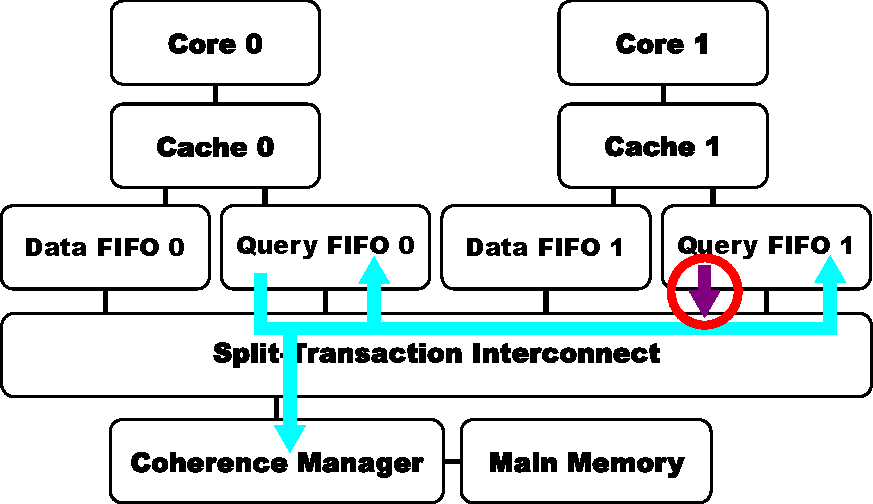
\includegraphics[width=0.6\textwidth]{\chapterdirectory/../second_intro/figure/demo_arch0.pdf}
\end{center}
\caption{Example of Interference}
\label{fig:second_intro:interference_example}
\end{figure}

\begin{example}[Example of Interference]
\label{ex:second_intro:interference}
In a system in which two cores, with one cache each, both attempting to send a
query to load data simultaneously, the interconnect will end up having to
choose one of the two queries to send first, and will put the other query in
waiting. This waiting lengthens the execution time of the associated
instruction and would not occur if there was no concurrent query, thus making
it an interference. Figure~\ref{fig:second_intro:interference_example}
illustrates this example, by having \textit{Cache 1}'s query be prevented
access to the interconnect during the other query's propagation, meaning that
the application running on \textit{Core 0} is interfering with the one running
on \textit{Core 1}.
\end{example}

%%\section{Context}
The ever increasing complexity of aircraft and the market's depreciation of
single-core processors are motivating the introduction of multi-core processors
in aeronautical systems.

The operation of a safety critical system requires its certification by the
relevant authorities. This certification is obtained through a process in which
an applicant argues for the compliance of that system with regulation. The
introduction of a new category of hardware in such a system renders this process
particularly difficult, as it implies a lack of preexisting process for the
generation of a proof of compliance. Furthermore, the link between this new
hardware and the high level certification objectives may not be obvious.

For multi-core processors aboard an aircraft, the certification authorities
have published a set of guidelines (\cite{cast32A}) on low level certification
objectives that the applicant ought to prove their use of the multi-core
processor fulfills. This document does not, however, provide guidance on how to
obtain proof that these objectives are fulfilled, nor exactly what parts of the
multi-core processor may be involved in ensuring or impeding each of these
objectives.

The analysis of multi-core processors is made difficult by their inherently
parallel nature. Users have little control over the minutiae of the order in
which operations are performed. Furthermore, the users may not even be aware of
all the operations involved as, with few exceptions, the documentation provided
by the manufacturers is insufficient to properly understand the inner workings
of processor components. This is especially true in the case of some components
who have huge impacts on the processor's performance and for which the actual
behavior is kept secret, seemingly to avoid copy by a competing manufacturer.
While having the applicant manufacture their own processor would resolve this
issue, it is not economically viable in the aeronautical domain. Thus, the use
of preexisting commercially available components (\textit{Commercial
Off-The-Shelf}, \textit{COTS}) is prevalent.

Because of this lack of documentation despite their complexity, the behavior of
multi-core processors is generally conceived to be undeterministic, and its
features are deactivated in order to make executions more predictable. Indeed,
while mechanisms such as prefetching, out-of-order execution, and so many
others offer a very much welcomed improvement of performances in most cases,
they still can lead to decreased performances in some rare cases. To ascertain
compliance in all cases, applicants are expected to validate their programs
using their \textit{Worst Case Execution Time} (\textit{WCET}), which is
generally negatively impacted by such optimizations.

Cache coherence is one such optimization. In most cases, it speeds up access to
data used by multiple cores and ensures that the changes on the data performed
by one core are propagated to the others. This requires coordination between
the caches. This coordination is performed automatically and takes over the
fetching of data from the system's main memory. As a result, the speed at which
a core accesses data is dependent on the actions performed by the other cores.
Indeed, not only can the content of each core's cache be altered because of the
actions of another, but the speed at which each cache fetches data is dependent
on the data found in the other caches. This impact on the performance (and,
potentially, the correctness) of one core by the actions of another is called
\textit{interference}.

\todomsg{%
Interference w/o CTRL from user's bad. Breaks software isolation, can't just
analyze each software separately.
}

\todomsg{%
Cache Coordination is complex. Current works simply recommend disabling it.
With shared data between cores, that's pretty much either re-implementing it
yourself (error prone, costly, or non-COTS) or disabling caches (perf worse
than with a single core processor).
}

This thesis proposes a strategy that lets the applicant be aware of
the interference generated by cache coherence in a COTS multi-core system, thus
allowing them to take control of it so that they may prove their system to be
compliant despite its use of cache coherence.

This strategy is composed of three steps:
\todomsg{Turns these into something more like: the objective of this step
was to\ldots, also, mention that some of this stuff was published in a paper.}
\begin{itemize}
\item
The first step, presented in
Chapter~\ref{chap:identifying_cache_coherence}, is meant to ensure the
applicant is fully aware of all the peculiarities of the cache coherence
protocol implemented by the multi-core architecture of their choice. To achieve
this, the applicant is asked to start by formalizing what they believe the
cache coherence protocol to be, in a fashion that leaves no possible ambiguity.
This hypothetical cache coherence protocol ought to be proved correct prior to
its comparison with the one actually implemented by the platform. Indeed, this
comparison is done through a series of simple benchmarks which, by themselves,
would leave some gaps in the applicant's knowledge of the architecture's cache
coherence protocol. The hypothetical cache coherence protocol fills these gaps
with something that is at the very least plausibly what ought to have been
found.

\item
From the previous step, the applicant obtained an ambiguity-free cache
coherence protocol corresponding to the one used by the targeted multi-core
architecture. However, the analysis of the protocol by itself does not reveal
much. In Chapter~\ref{cha:modeling_cache_coherence}, the applicant is thus
invited to create a model of the cache coherence mechanisms in their entirety.
This thesis proposes a framework for the creation of such a model, basing
itself on networked timed automata. The components involved in maintaining
cache coherence all have their own automaton, letting the applicant model their
own system through the instantiation of the right amount of each type of
component as well as the setting of fairly basic parameters matching their
targeted architecture's documentation. Computer programs are also part of the
model, and are represented by sequences of instructions related to data
manipulation.

\item
The model created in the previous step can be used to perform an analysis of
the system. In this last step, Chapter~\ref{chap:exposing_interference}, are
proposed properties corresponding to the occurrence of interference, including
whether they had any impact, as well as some properties to measure said impact
on the execution time. Three types of interference are identified: Minor
interference, corresponding to the processing of other caches' queries without
impact on the studied cache; Demoting interference, where the studied cache
looses writing permissions because of another cache's query; and expelling
interference, where another cache's actions force the studied cache to evict a
memory element.
\end{itemize}


\section{The Issue of Cache Coherence}
\label{sec:intro:prob_statement}
When multiple cores make use of the same memory elements, separate copies of
these memory elements find themselves in different caches. As these copies are
separate, changes made to a copy are not reflected on the other copies. This
makes parallel computing difficult: a core might not be using the most
up-to-date value of the shared memory elements and the modifications it performs
might be blindly overridden by another core.

Cache coherence refers to mechanisms that will ensure all these separate copies
stay consistent. In effect, it will ensure that there is never an ambiguity on
the current value of memory elements, and that any core accessing a memory
element is using this most up-to-date value.

Achieving cache coherence requires caches to coordinate with each other. This
is done through shared buses, on which caches send queries to communicate needs
and receive data messages in reply. These buses in themselves are thus a
heavily used shared resource, making it a source of interference. However, the
main cause of cache coherence interference is that, to maintain coherence, these
queries can force caches to lose access to some of their content. As a result,
the actions of another core will determine whether a core can find the memory
element it wants through a quick cache access or if this will require a time
consuming fetch.

These cache coherence mechanisms are generally fully automated, meaning that
the application developers do not directly control when cache queries are made.
This makes predicting the emission and effects of these queries difficult.
Indeed, the emission of a query is determined by both program instruction and
the content of the cache, and the latter is subject to uncontrolled
modifications by queries emitted from other caches. This makes cache coherence
a source of important execution time variations and a challenge to
certification.

\section{Overview of the Thesis}
This thesis starts by introducing prerequisites: timed automata
(Chapter~\ref{cha:formal_methods}) and cache
coherence (Chapter~\ref{cha:cache_coherence}).
Once these have
been presented, the focus of this thesis can be explained in full
(Chapter~\ref{cha:second_intro}).
Indeed, The purpose of the thesis is to
develop a framework to ensure the applicant is made aware of the interference
generated by cache coherence in their chosen COTS multi-core processor.

To determine the state of the art and what specifically needs to be developed,
a whole part is dedicated to the relevant existing literature.
First is architecture profiling, for which existing solutions
relying on benchmarks are presented in Chapter~\ref{cha:micro-benchs}, including
works with a focus on caches. The current practices with regards to the use of
caches in multi-core employed in critical environments are detailed in
Chapter~\ref{cha:handling_it}. Since the solution proposed in this thesis
relies on formal methods, a number of existing works that have a similar
approach to the study of architectures are presented in
Chapter~\ref{cha:analyzing_rel_work}.

After clarifying what is left to be done to achieve a full framework that will
help with the cache coherence part of the certification, this thesis proposes
three contributions: a strategy to properly identify an architecture's cache
coherence protocol, a model template for multi-core architectures with cache
coherence support, and analyses to be performed on instantiated models in order
to expose the interference.
\begin{itemize}
\item
The first contribution, presented in
Chapter~\ref{chap:identifying_cache_coherence}, is meant to ensure the
applicant is fully aware of all the peculiarities of the cache coherence
protocol implemented by the multi-core architecture of their choice. To achieve
this, the applicant is asked to start by formalizing what they believe the
cache coherence protocol to be, in a fashion that leaves no possible ambiguity.
This hypothetical cache coherence protocol is then validated against the
architecture through observations made with micro-benchmarks.

\item
Using the previous contribution, the applicant obtained an ambiguity-free cache
coherence protocol corresponding to the one used by the targeted multi-core
architecture. However, the analysis of the protocol by itself does not reveal
much. The second contribution, presented in
Chapter~\ref{cha:modeling_cache_coherence}, proposes the model of a multi-core
architecture to the applicant. This model, made of networked timed automata, is
meant to be instantiated to fit the applicant's chosen architecture, and can
automatically be made to use the aforementioned ambiguity-free cache coherence
protocol.

\item
The instantiated model created using the previous contribution can be used to
perform an analysis of interference occurring in the system. This third
contribution, presented in Chapter~\ref{chap:exposing_interference}, shows how
model checking can be employed to expose the causes and effects of cache
coherence interference in the system. The analyzes include worst-case execution
time estimation, as well as the identification of how each program instruction
is affected by and/or generates interference.
\end{itemize}

